% ****** Start of file apssamp.tex ******
%
%   This file is part of the APS files in the REVTeX 4 distribution.
%   Version 4.0 of REVTeX, August 2001
%
%   Copyright (c) 2001 The American Physical Society.
%
%   See the REVTeX 4 README file for restrictions and more information.
%
% TeX'ing this file requires that you have AMS-LaTeX 2.0 installed
% as well as the rest of the prerequisites for REVTeX 4.0
%
% See the REVTeX 4 README file
% It also requires running BibTeX. The commands are as follows:
%
%  1)  latex apssamp.tex
%  2)  bibtex prb
%  3)  latex apssamp.tex
%  4)  latex apssamp.tex
%
%\documentclass[aps,prb,preprint,groupedaddress,showpacs]{revtex4-1}
\documentclass[aps,prl,preprint,superscriptaddress]{revtex4}
%\documentclass[aps,prl,twocolumn,superscriptaddress]{revtex4}
%\documentclass[aps,prl,twocolumn,superscriptaddress]{revtex4}
%\documentclass[aps,prb,twocolumn,groupedaddress]{revtex4-1}


%\documentclass[twocolumn,showpacs,preprintnumbers,amsmath,amssymb]{revtex4}
%\documentclass[preprint,showpacs,preprintnumbers,amsmath,amssymb]{revtex4}

% Some other (several out of many) possibilities
%\documentclass[preprint,aps]{revtex4}
%\documentclass[preprint,aps,draft]{revtex4}
%\documentclass[prb]{revtex4}% Physical Review B

\usepackage{graphics}
\usepackage{graphicx}% Include figure files
\usepackage{epstopdf}
\usepackage{dcolumn}% Align table columns on decimal point
\usepackage{bm}% bold math
\usepackage{amsmath}
\usepackage{amssymb}
\usepackage{latexsym}
\usepackage{epsfig}
\usepackage{amsbsy}
\usepackage{array}
\usepackage{amssymb}
\usepackage{setspace}
\usepackage{bm}
\usepackage{float}
\usepackage[caption = false]{subfig}

\newcommand{\ssint}{ - \!\!\!\!\! \int }
\def\sint{\ifmmode{- \!\!\!\!\!\! \int}
    \else{\hbox{$- \!\!\!\! \int \ $}}\fi}


\newcommand{\bsigma}{\boldsymbol{\sigma}}
\newcommand{\bmu}{\boldsymbol{\mu}}
\newcommand{\bvepsilon}{\boldsymbol{\varepsilon}}
\newcommand{\bepsilon}{\boldsymbol{\epsilon}}
\newcommand{\balpha}{\boldsymbol{\alpha}}
\newcommand{\bkappa}{\boldsymbol{\kappa}}
\newcommand{\bchi}{\boldsymbol{\chi}}
\newcommand{\bgamma}{\boldsymbol{\gamma}}
\newcommand{\bpsi}{\boldsymbol{\psi}}
\newcommand{\bnu}{\boldsymbol{\nu}}
\newcommand{\bzero}{\boldsymbol{0}}
\newcommand{\bbeta}{\boldsymbol{\beta}}
\newcommand{\bSigma}{\boldsymbol{\Sigma}}

\newcommand{\va}{\varphi}
\newcommand{\ep}{\epsilon}
\newcommand{\mbf}{{\bf m}}
\newcommand{\pbf}{{\bf p}}
\newcommand{\xbf}{{\bf x}}
\newcommand{\weak}{\rightharpoonup}
\newcommand{\rgoto}{\rightarrow}

\newcommand{\grad}{\mbox{grad}}
\newcommand{\curl}{\mbox{curl}}
\newcommand{\dive}{\mbox{div}}


\newcommand{\tr}{\mbox{tr}}

\newcommand{\ba}{\mathbf{a}}
\newcommand{\bb}{\mathbf{b}}
\newcommand{\bc}{\mathbf{c}}
\newcommand{\bd}{\mathbf{d}}
\newcommand{\be}{\mathbf{e}}
\newcommand{\bsf}{\mathbf{f}}
\newcommand{\bg}{\mathbf{g}}
\newcommand{\bsi}{\mathbf{i}}
\newcommand{\bk}{\mathbf{k}}
\newcommand{\bn}{\mathbf{n}}
\newcommand{\bo}{\mathbf{o}}
\newcommand{\bp}{\mathbf{p}}
\newcommand{\bq}{\mathbf{q}}
\newcommand{\br}{\mathbf{r}}
\newcommand{\bs}{\mathbf{s}}
\newcommand{\bt}{\mathbf{t}}
\newcommand{\bu}{\mathbf{u}}
\newcommand{\bv}{\mathbf{v}}
\newcommand{\bw}{\mathbf{w}}
\newcommand{\bx}{\mathbf{x}}
\newcommand{\by}{\mathbf{y}}
\newcommand{\bz}{\mathbf{z}}

\newcommand{\bca}{\mathbf{A}}
\newcommand{\bcb}{\mathbf{B}}
\newcommand{\bcc}{\mathbf{C}}
\newcommand{\bcd}{\mathbf{D}}
\newcommand{\bce}{\mathbf{E}}
\newcommand{\bcf}{\mathbf{F}}
\newcommand{\bcg}{\mathbf{G}}
\newcommand{\bch}{\mathbf{H}}
\newcommand{\bck}{\mathbf{K}}
\newcommand{\bcj}{\mathbf{J}}
\newcommand{\bci}{\mathbf{I}}
\newcommand{\bcl}{\mathbf{L}}
\newcommand{\bcm}{\mathbf{M}}
\newcommand{\bcn}{\mathbf{N}}
\newcommand{\bco}{\mathbf{O}}
\newcommand{\bcp}{\mathbf{P}}
\newcommand{\bcq}{\mathbf{Q}}
\newcommand{\bcr}{\mathbf{R}}
\newcommand{\bcs}{\mathbf{S}}
\newcommand{\bct}{\mathbf{T}}
\newcommand{\bcu}{\mathbf{U}}
\newcommand{\bcv}{\mathbf{V}}
\newcommand{\bcw}{\mathbf{W}}
\newcommand{\bcx}{\mathbf{X}}
\newcommand{\bcz}{\mathbf{Z}}
\newcommand{\bcy}{\mathbf{Y}}

%\nofiles

\begin{document}
	
	
	\title{Predator-Prey Model}% Force line breaks with \\
	
	\author{Connor Hann, Xiaomeng Jia, Peifan Liu and Xinyu Wu}
	\affiliation{Physics Department, Duke University}
	
	
	\date{\today}
	
	\begin{abstract}
		To be added.
	\end{abstract}
	
	\maketitle
	
	
	
	\section{Background} 
Modeling the interactions between predator and prey is a question of great ecological importance, as accurate models can allow one to make reliable predictions and thereby inform decisions in conservation, habitat preservation, hunting regulations, etc. There exist a variety of methods for modeling the interactions between predator and prey, and these models, though simple, are often in quite good agreement with what is observed. Take the classic Lotka-Volterra Model as an example. While this model is nothing more than a set of first-order nonlinear differential equations that one may solve numerically for a particular set of initial conditions, the model is capable of providing a qualitatively accurate description of the data, as is shown in Fig.~\ref{LV}. 

\begin{figure}[H]
	\centering
	\subfloat{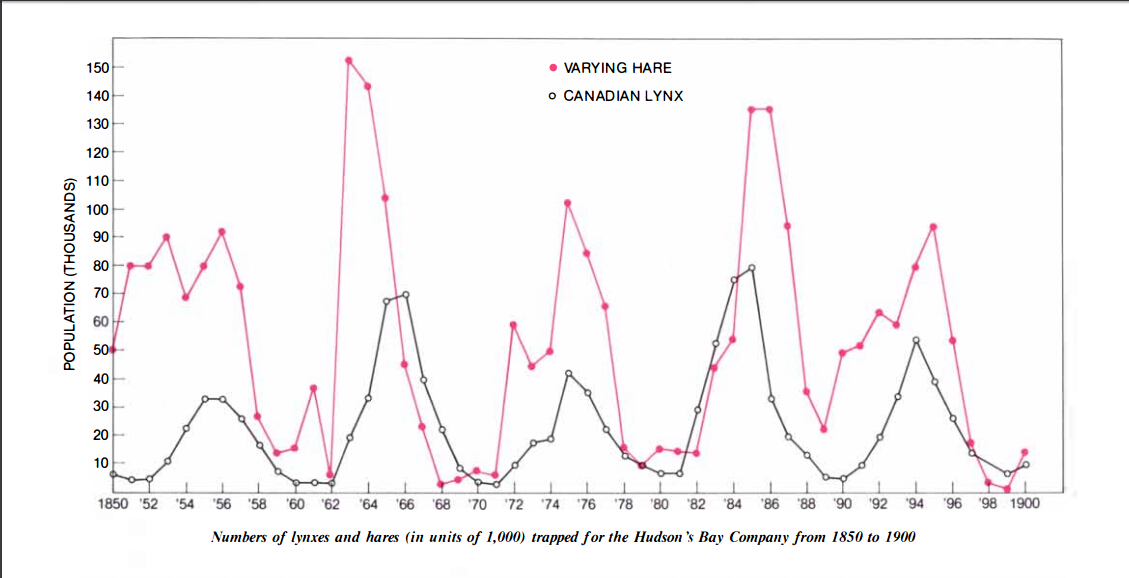
\includegraphics[width = 0.7\textwidth]{LV_data}}\\
	\subfloat{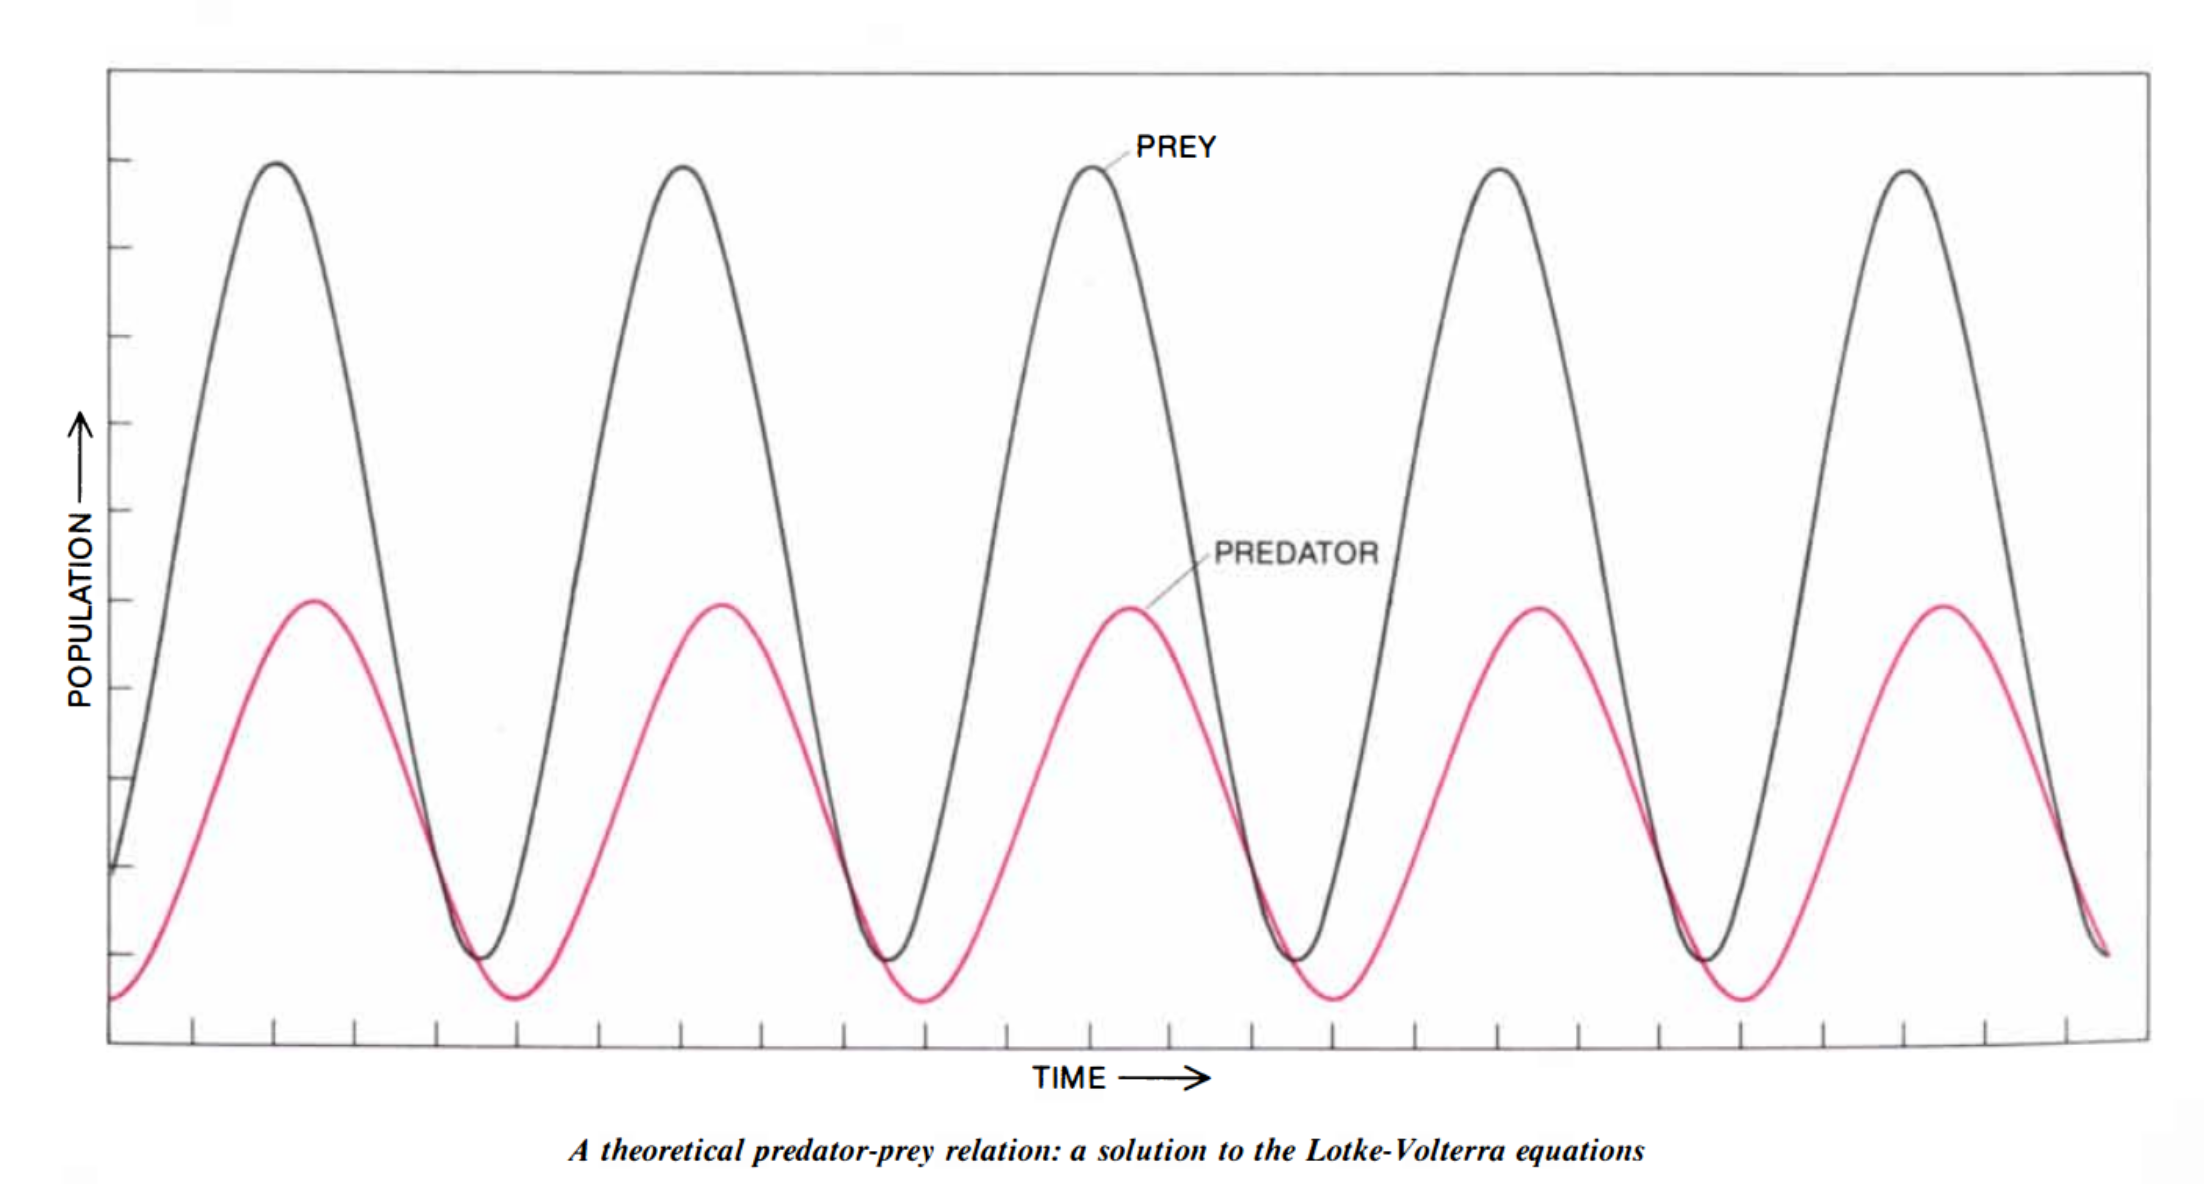
\includegraphics[width = 0.7\textwidth]{LV_prediction}}
	\caption{(Top) experimental data of Hare and Lynx populations, (Bottom) predictions from the Lotka-Volterra equations. }
	\label{LV} 
\end{figure}

In this work we study the behavior of a slightly different model, one that  is similar to the Lotka-Volterra Model in that it consists of only a simple set of rules, but the nature of the actual simulation is quite different. In our case, we consider two populations, sharks and fish living on a two-dimensional lattice. We simulate the movement and behavior of each shark and fish individually and can observe fluctuations of the two populations as a function of time. Unlike the Lotka-Volterra Model, however, we are able to see exactly where all of the sharks and fish are and this allows us to attain a deeper understanding of what causes the fluctuations in populations and the conditions that may lead to extinction. 
	
	\section{Implementation}
	
	\section{Numerical Results}

\begin{figure}[H]
	\centering
	\subfloat{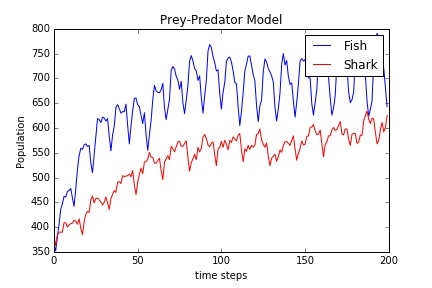
\includegraphics[width = 0.5\textwidth]{fish10shark15starve8}}
	\subfloat{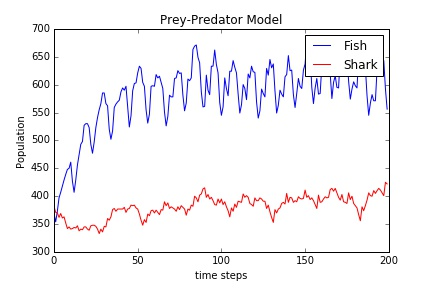
\includegraphics[width = 0.5\textwidth]{fish10shark25starve8}}\\
	\subfloat{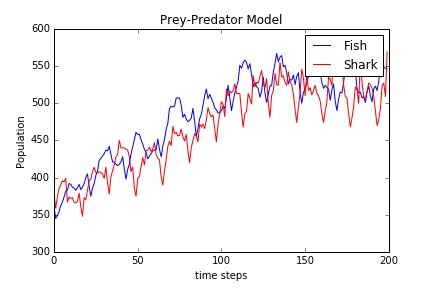
\includegraphics[width = 0.5\textwidth]{fish20shark15starve8}}
	\subfloat{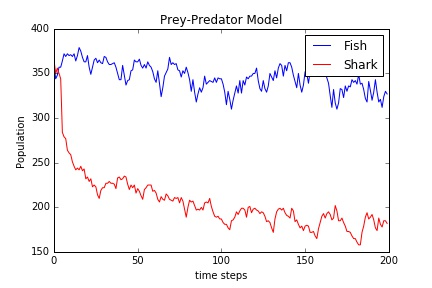
\includegraphics[width = 0.5\textwidth]{fish20shark25starve5}}
	\caption{Other typical clusters grown using the DLA method}
	\label{more_clusters} 
\end{figure}
 
 \section{Conclusion}
  
\end{document}
	
	%
	% ****** End of file apssamp.tex ******
